\chapter{hep_c}
\label{applications-rfx}

Hepatitis C is a viral infection that attacks the liver.  In a small portion of acute cases, the body can eliminate the virus; however the majority of acute cases develop into chronic infections [1].  Chronic infections cause liver damage and may develop to end stage liver disease or cirrhosis.  Few, if any, chronic cases experience symptoms and only one third of acute cases are symptomatic and jaundice.  Chronic symptoms are nonspecific, intermittent and mild with the most common symptom being fatigue [2, 1].  Common symptoms for severe and advanced disease stages include nausea, dark urine and jaundice [1].  Since hepatitis C infections are asymptomatic, diagnosis requires laboratory testing for both hepatitis antibodies (anti-HCV) and the hepatitis virus (HCV RNA) [2].  There is no vaccination for hepatitis C, but therapy can prevent advanced liver disease [3].

Compared to other countries in the region, Egypt has a high hepatitis C prevalence.  In an attempt to treat endemic schistosomiasis, a common parasitic worm that affects the urinary tract, gut and liver, the Egyptian Ministry of Health launched widespread injection-based treatment throughout 1950-1980.  While there were improvements in schistosomiasis-induced mortality, recycled needles and poor needle sterilization infected many with hepatitis C [4, 5, 6].  The spatial variations of hepatitis C in North Africa and the Middle East make it an excellent example of hierarchical random effects modeling.

Random effects modeling detects systematic differences among different hierarchies, or levels, of data.  The spatial hierarchy in the GBD 2010 study uses countries nested in regions nested in super-regions.  There are 21 regions defined by demographic and epidemiological similarities that are further clustered by 7 super-regions.

The analysis of hepatitis C uses anti-HCV prevalence data to compare hepatitis C infection levels globally.  Data without measures of uncertainty (effective sample size, standard error or 95\% confidence intervals) and duplicated data from different sources are excluded from analysis.  Also excluded were incomplete data or data from high-risk populations [3].

    \begin{figure}[h]
        \begin{center}
            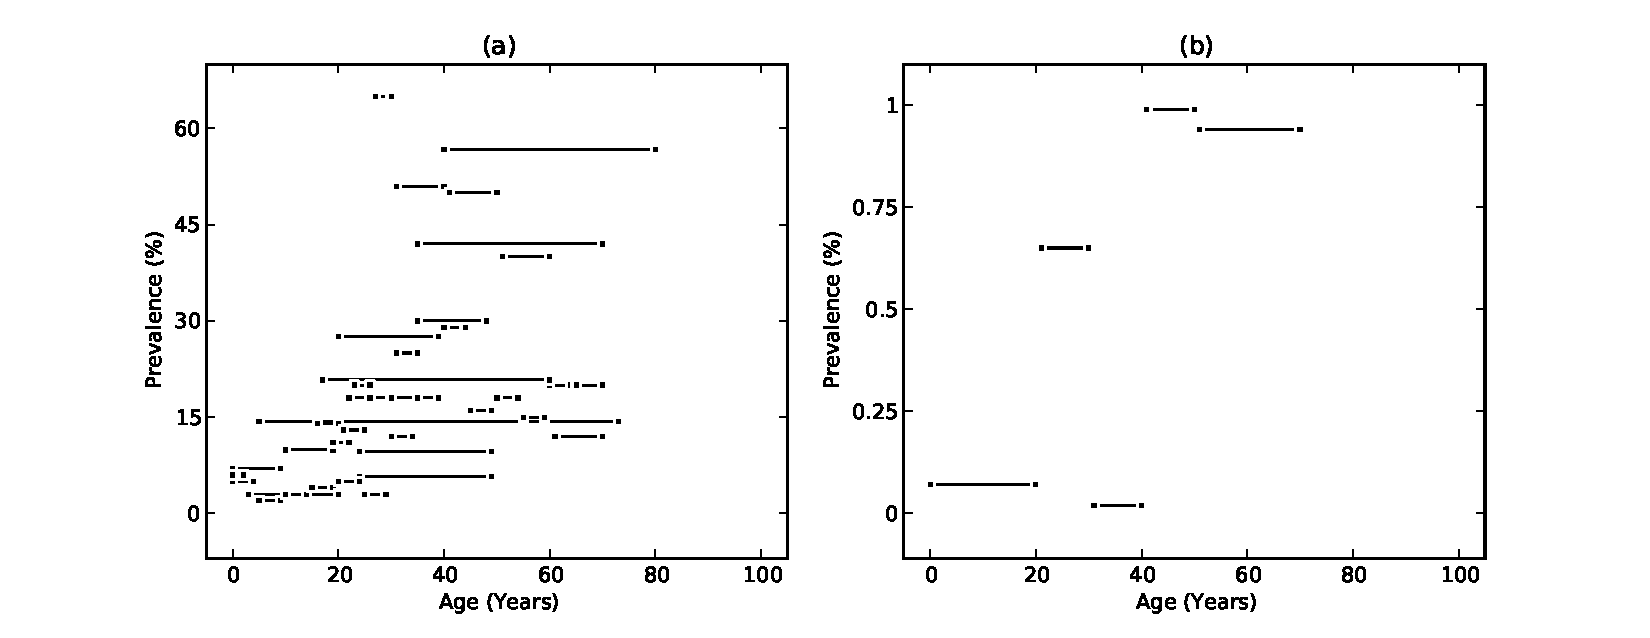
\includegraphics[width=\textwidth]{hepc-data_EGY_v_JOR.pdf}
            \caption{Prevalence data included for the modeling of hepatitis C.  Panel (a) shows Jordan and panel (b) Egypt.  Notice that hepatitis C prevalence in Egypt is approximately 7 times that of the Jordan, even though they are both in the region of Northern Africa and the Middle East.}
            \label{fig:app-hepc data}
        \end{center}
    \end{figure}

The analysis uses an age-standardizing hierarchical random effects generalized negative binomial spline model to estimate prevalence.  The hierarchical random effects allow the model to capture variation in the region of North Africa and the Middle East.  Looking at the table below, Egypt (EGY) has significantly higher prevalence than the other countries in the region.  Figure ?.?, confirms this as the estimate for Egypt is much above the regional average.

\begin{table}[h]
        \begin{center}
        \caption{ Hepatitis C prevalence estimations from random effects model in the region of North Africa and the Middle East}
        \label{tab:hepc regional rfx}
        \begin{tabular}{|l|c|}
            \hline
                Country & Posterior Mean & Lower 95\% HPD  & Upper 95\%  HPD \\
            \hline
                EGY	&	1.88	&	1.6,	&	2.2	\\
                JOR	&	-0.59	&	-1.0,	&	-0.1	\\
                SAU	&	-0.76	&	-1.1,	&	-0.4	\\
                IRQ	&	0.07	&	-0.4,	&	0.5	\\
                IRN	&	0.00	&	-0.5,	&	0.4	\\
                YEM	&	0.05	&	-0.4,	&	0.5	\\
                TUR	&	-0.31	&	-0.6,	&	0.1	\\
                SYR	&	-0.16	&	-0.7,	&	0.3	\\
                TUN	&	-0.19	&	-0.7,	&	0.3	\\
            \hline
        \end{tabular}
        \end{center}
    \end{table}

    \begin{figure}[h]
        \begin{center}
            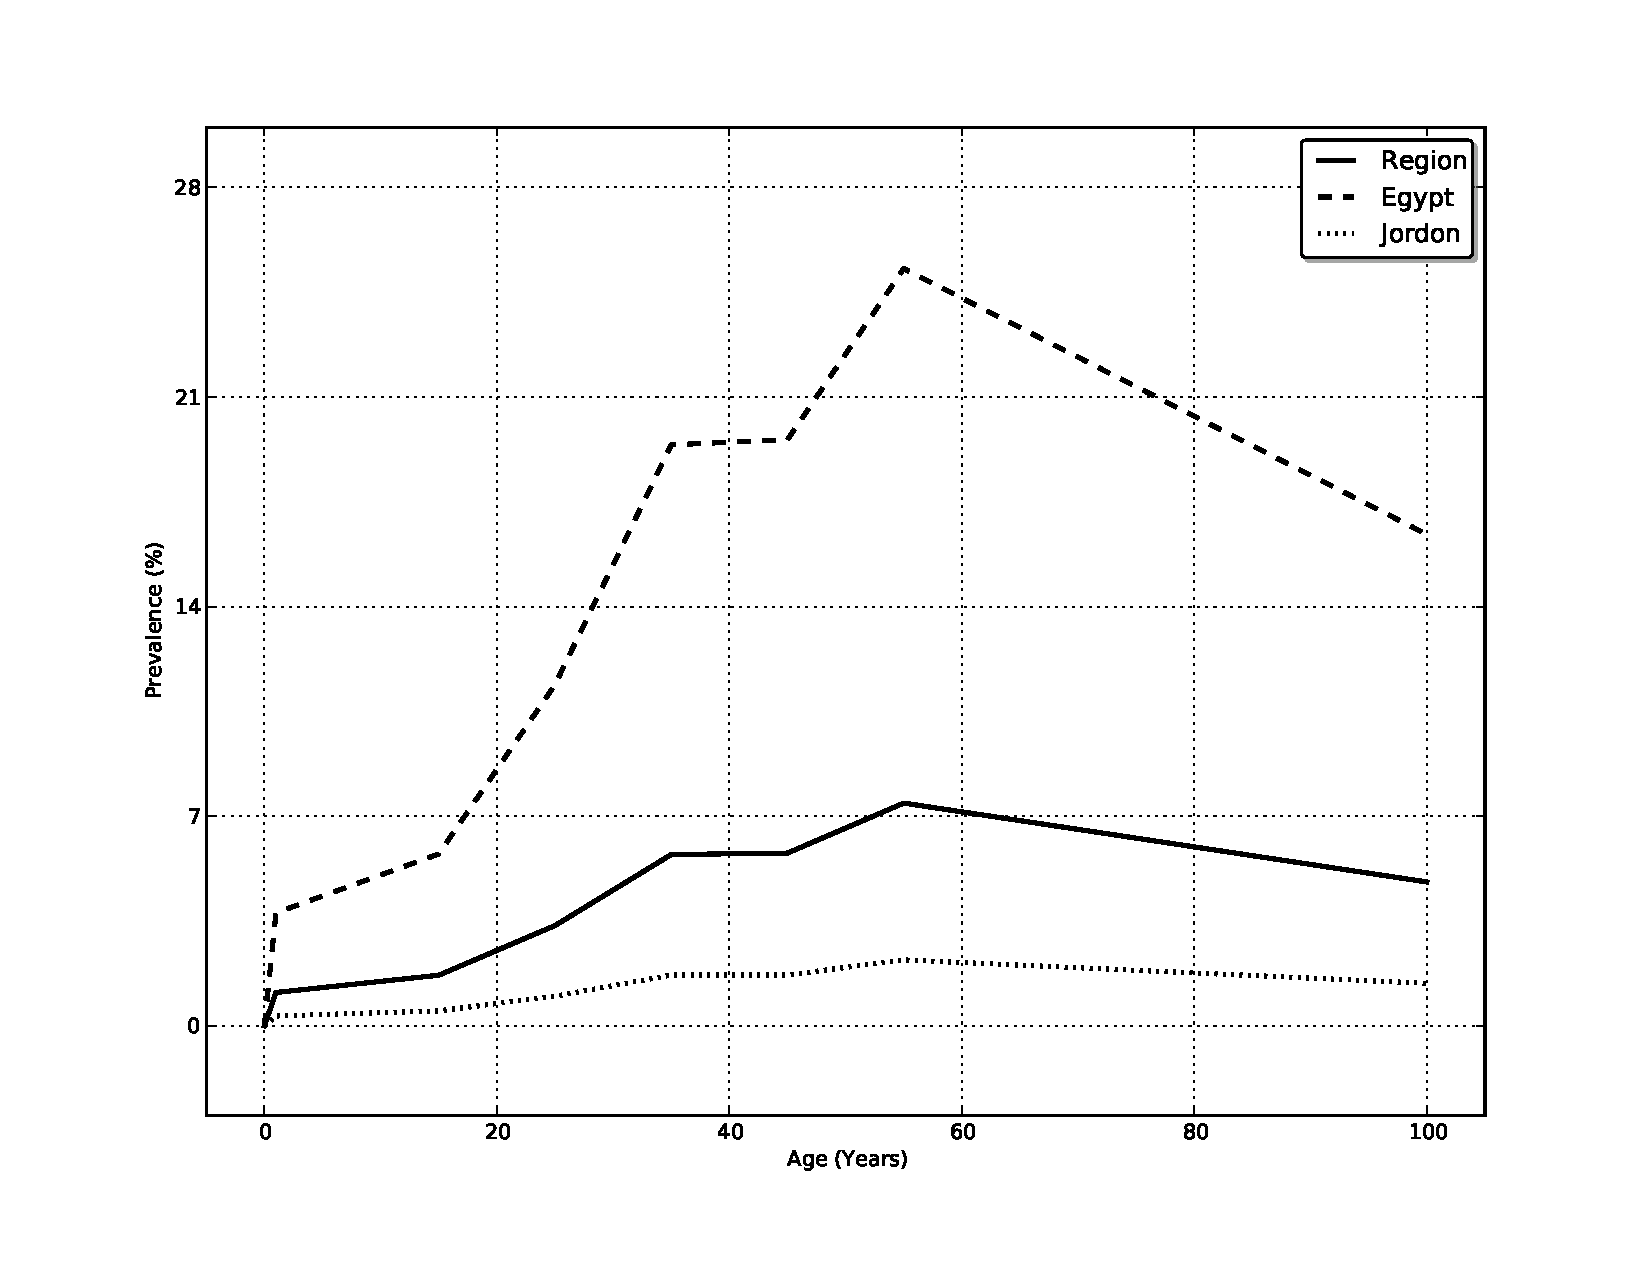
\includegraphics[width=\textwidth]{hepc-region_v_EGY_v_JOR.pdf}
            \caption{The 1990 estimate of hepatitis C prevalence for men in the region of North Africa and Middle East and the countries Egypt and Jordan.  These estimates only use 2 levels in the hierarchal random effects model-region and country.}
            \label{fig:app-hepc regional rfx}
        \end{center}
    \end{figure}    

In such noisy data, placing a prior on the dispersion of the data informs the model of the data heterogeneity.  This allows the model to infer how dispersed the random effects are between geographic regions, and hence quantify the uncertainty in the geographic regions for which no data is available.  Changing the prior for the heterogeneity of the global data has effects on the country level as seen in the figure below.  Random effects modeling detects within sample variation and true variation that cannot be explained by a covariate.  Therefore, a change in the prior on global heterogeneity changes the level of variation and thus the random effect size.  As seen in the figure below, when the prior on global heterogeneity is 'very', the estimates are compressed.

better discussion of compression needed.

    \begin{figure}[h]
        \begin{center}
            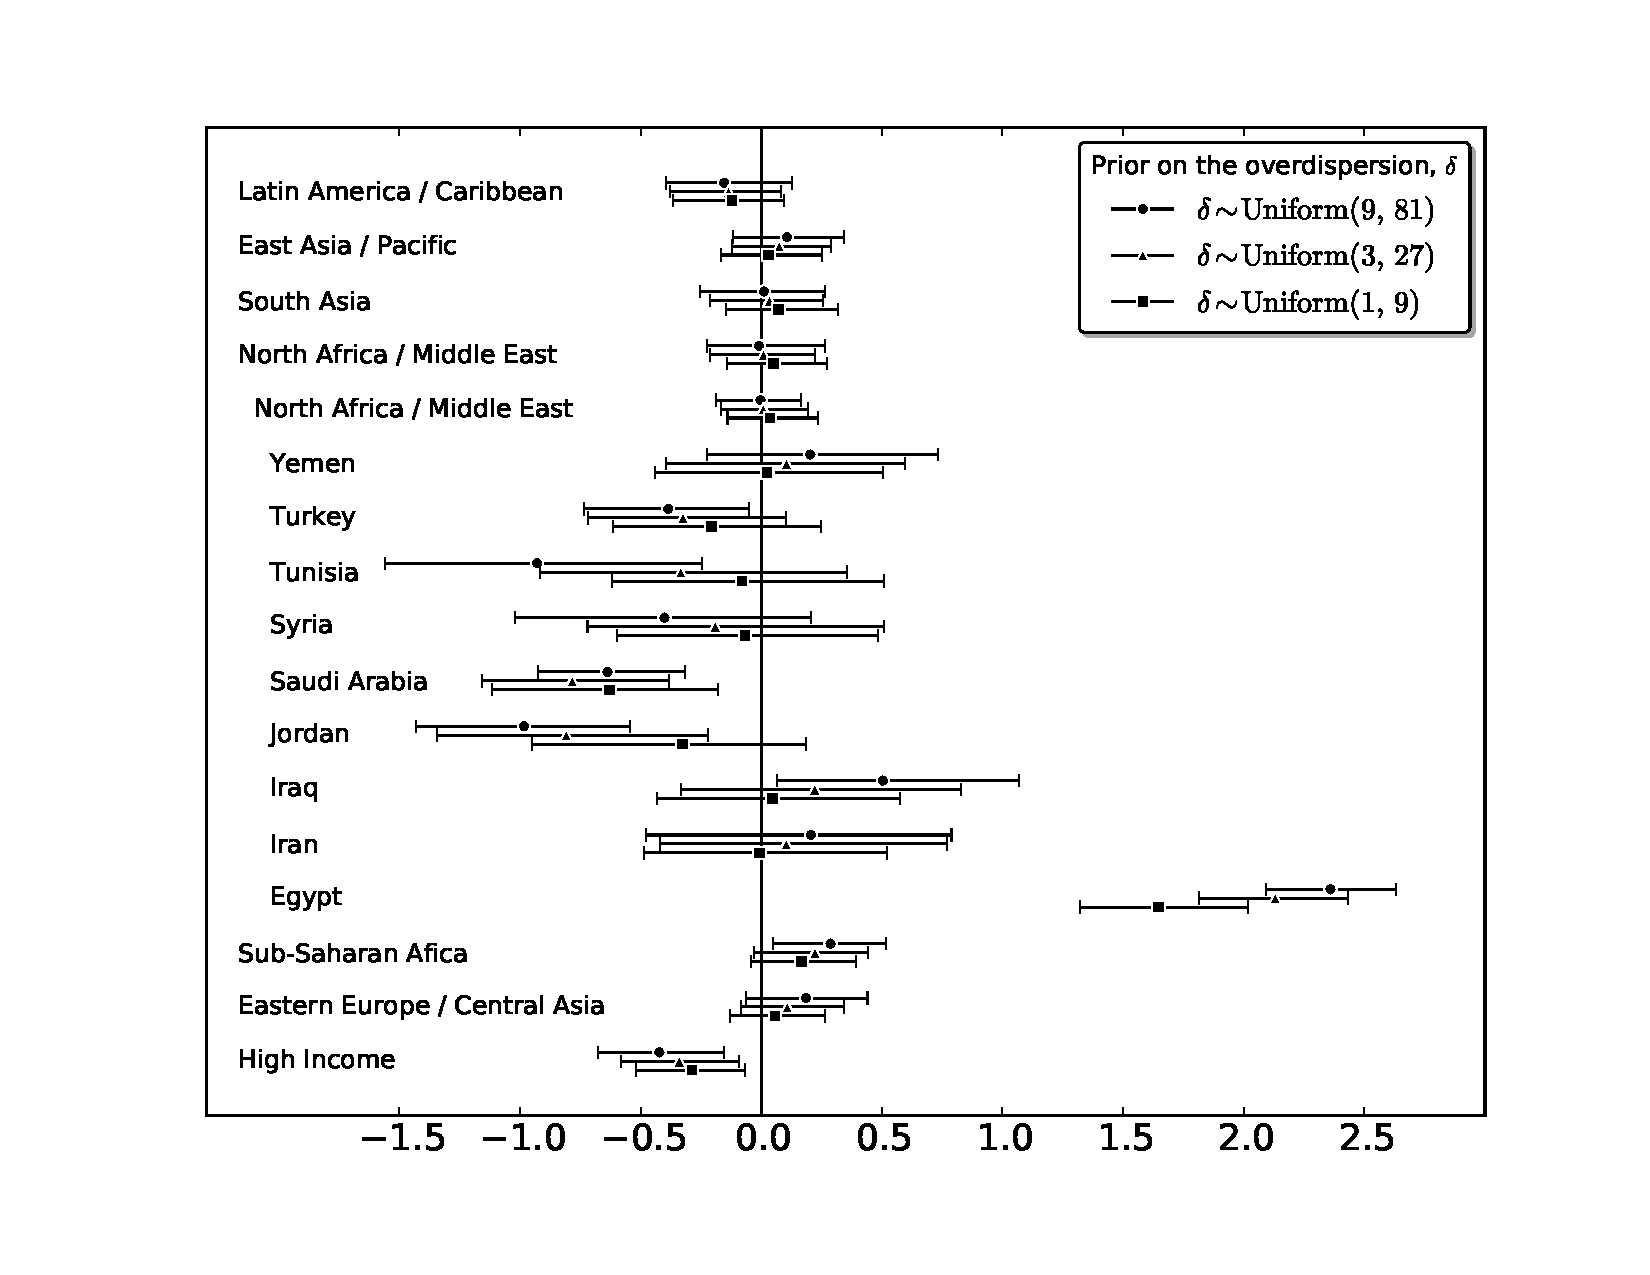
\includegraphics[width=\textwidth]{hepc-tree_plot_global_hetero.pdf}
            \caption{The 1990 intercept shift of hepatitis C prevalence  in log space for men with different priors on global heterogeneity, (a) 'slightly', (b) 'moderately' and (c) 'very').  Four levels (global, super-region, region, country) were used in the hierarchal model random effects model.  Notice that changes for in the prior on global data heterogeneity affects the estimates at the country level (****) the most.}
            \label{fig:app-hepc global hetero}
        \end{center}
    \end{figure}
